
\begin{center}
\Huge
Monotoniforhold og ekstrema
\end{center}
\section*{Monotoniforhold}
\stepcounter{section}
Vi siger, at en funktion er monoton på et interval, hvis den enten er voksende eller aftagende på intervallet. Mere præcist har vi følgende definition.
\begin{defn}
En funktion $f$ siges at være voksende på et interval $I$, hvis det for alle $x_1,x_2$ i $I$ gælder, at 
\begin{align*}
x_1<x_2 \ \Rightarrow \ f(x_1)\leq f(x_2).
\end{align*}
Hvis der tilmed gælder, at 
\begin{align*}
x_1<x_2 \ \Rightarrow \ f(x_1)<f(x_2),
\end{align*}
så siges funktionen at være strengt voksende på $I$. 

En funktion $f$ siges at være aftagende på et interval $I$, hvis det for alle $x_1,x_2$ i $I$ gælder, at 
\begin{align*}
x_1<x_2 \ \Rightarrow f(x_1)\geq f(x_2).
\end{align*}
Hvis der tilmed gælder, at 
\begin{align*}
x_1<x_2 \ \Rightarrow f(x_1)>f(x_2),
\end{align*}
så siges funktionen at være strengt aftagende på $I$.
\end{defn}
Monotoniforhold omhandler at finde de intervaller, hvor en funktion er enten voksende eller aftagende. 

Vi vil starte med at definere, hvad et lokalt ekstremum er
\begin{defn}
En funktion $f$ siges at have et lokalt maksimum i $x_0$, hvis der i en omegn $I$ af $x_0$ gælder, at 
\begin{align*}
x\in I,x\neq x_0 \ \Rightarrow\  f(x)<f(x_0).
\end{align*} 
Hvis $I$ kan vælges som hele definitionsmængden af $f$, så siges $x_0$ at være et globalt maksimum.


En funktion $f$ siges at have et lokalt minimum i $x_0$, hvis der i en omegn $I$ af $x_0$ gælder, at 
\begin{align*}
x\in I,x\neq x_0 \ \Rightarrow\ f(x)>f(x_0).
\end{align*}
Hvis $I$ kan vælges som hele definitionsmængen af $f$, så siges $x_0$ at være et globalt minimum.
\end{defn}

Vi kan se ekstremumspunkterne af en funktion $f$ på Fig. \ref{fig:ekstremum}
\begin{figure}[H]
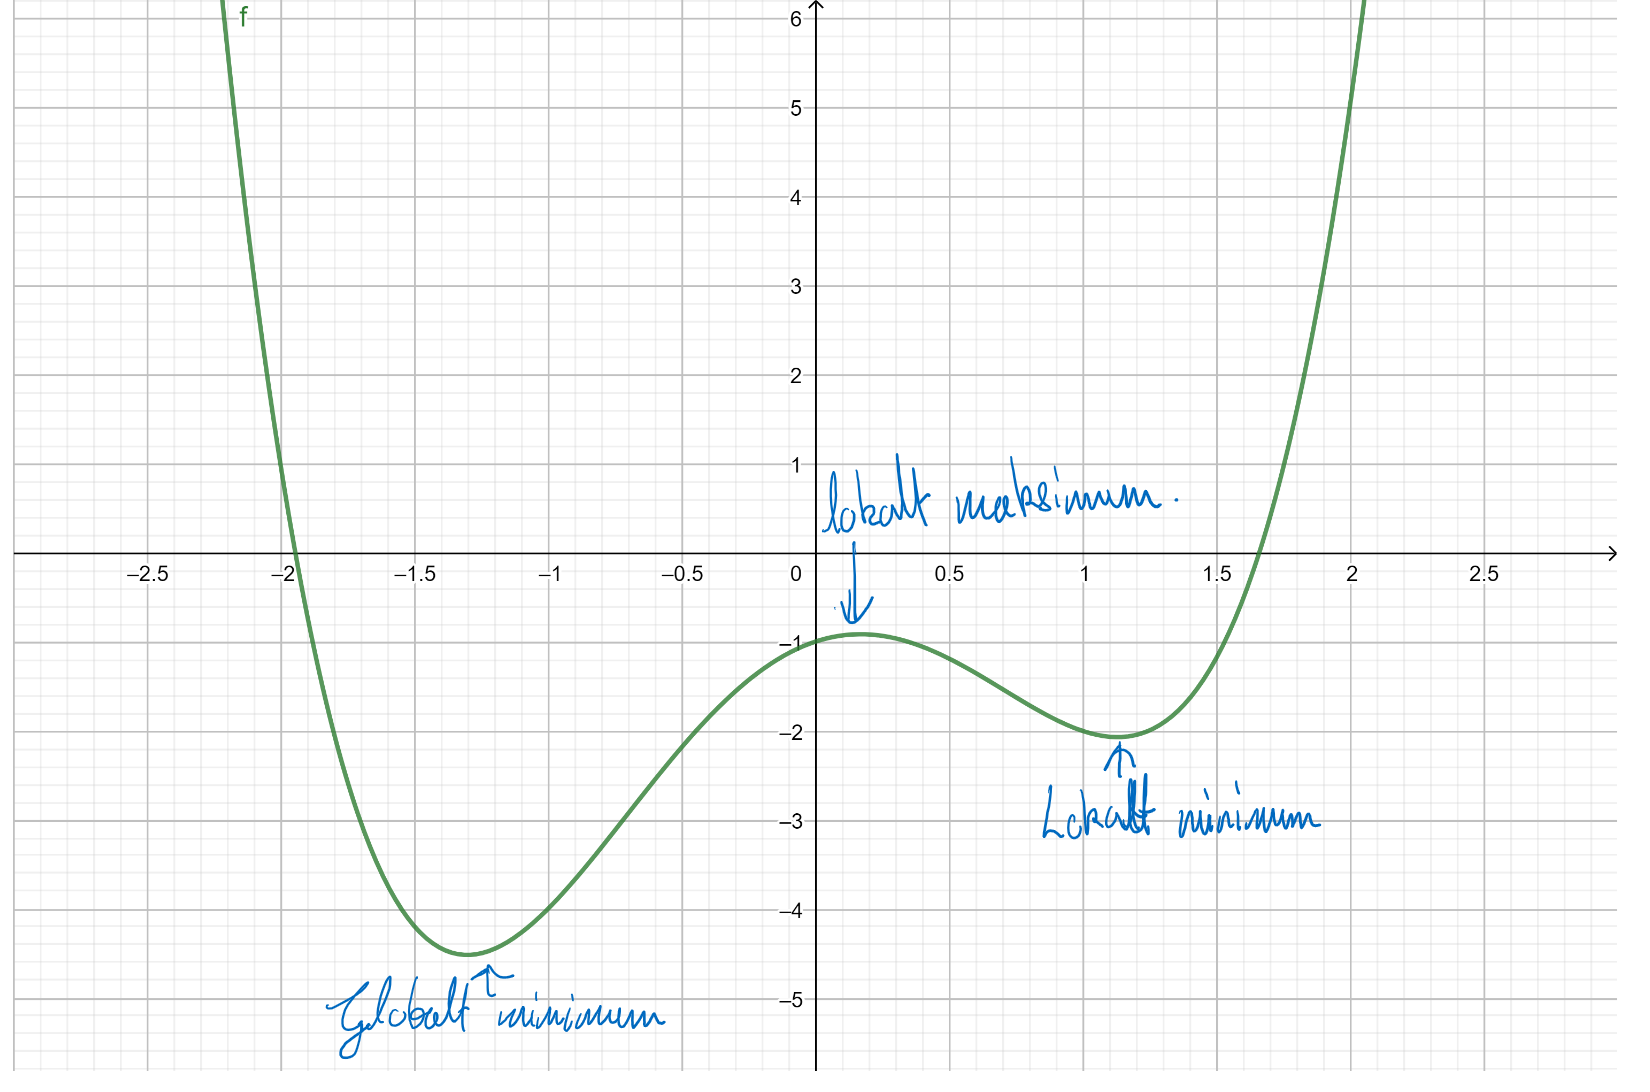
\includegraphics[width=\textwidth]{Billeder/ekstremum2.png}
\caption{Funktion med angivne ekstremumspunkter.}
\label{fig:ekstremum}
\end{figure}
Et maksimum og minimum kaldes for et ekstremumspunkt.
For at finde ekstremumspunkter, kan vi udnytte følgende sætning:
\begin{setn}
En funktion $f$ har ekstremum i et punkt $x_0$ kun hvis $f'(x_0) = 0$.
\end{setn}
\begin{exa}
Funktion, der er plottet i Fig. \ref{fig:ekstremum} har forskrift
\begin{align*}
f(x) = x^4-3x^2+x-1.
\end{align*}
Vi bestemmer $f'(x) = 4x^3-6x+1$. Denne sætter vi lig nul:
\begin{align*}
4x^3-6x+1 = 0,
\end{align*}
og får $x \approx -1.3 \ \vee\  x \approx 0.17 \ \vee \ x \approx 1.13$. 

Derfor har vi ekstremumspunkter
\begin{align*}
&(-1.3,f(-1.3)) = (-1.3,-4.51), &&(0.17,f(0.17)) = (0.17,-0.92),  \\ &(1.13,f(1.13))=(1.13,-2.07).
\end{align*} 
\end{exa}

\section*{Opgave 1}
Find ekstremumspunkterne for følgende funktioner:
\begin{align*}
&1) \ x^2    &&2) \ 3x^3+2x+1    \\
&3) \ 10 + 5x+ \sqrt{x}   &&4) \ \ln(x)\sqrt{x}   \\
&5) \  3x^2+\ln(x^2)  &&6) \  \ln(x^2)+3x^3  \\
&7) \ x^{5/2}-2x    &&8) \  e^{2x+3} +10x^2  \\
&9) \ x^{\ln(x)}   &&10) \  x^5+x^4+x^3+x^2-x+1  \\
\end{align*}
\section*{Opgave 2}
Plot funktionerne fra Opgave 1 omkring deres ekstremumspunkter og afgør i hvilke intervaller, de ser ud til at være voksende og aftagende.